\documentclass{article}
\usepackage[utf8]{inputenc}
\usepackage[margin=0.8in]{geometry}
\usepackage{amsmath}
\usepackage{graphicx}
\usepackage{amsthm}
\usepackage{algorithm}
\usepackage{algpseudocode}
\usepackage{enumitem}
\usepackage{verbatim}
\usepackage{color, soul}
\usepackage{tikz}

\graphicspath{ {./} }
% \usepackage{tikz-qtree}

\title{CS130A HW5}
\author{Matthew Ho}
\date{November 2021}

\usepackage{listings}
\usepackage{color}

\definecolor{codegreen}{rgb}{0,0.6,0}
\definecolor{codegray}{rgb}{0.5,0.5,0.5}
\definecolor{codepurple}{rgb}{0.58,0,0.82}
\definecolor{backcolour}{rgb}{0.95,0.95,0.92}

\lstdefinestyle{style1}{
    commentstyle=\color{codegreen},
    keywordstyle=\color{magenta},
    numberstyle=\tiny\color{codegray},
    stringstyle=\color{codepurple},
    basicstyle=\ttfamily\footnotesize,
    breakatwhitespace=false,         
    breaklines=true,                 
    captionpos=b,                    
    keepspaces=true,                 
    numbers=left,                    
    numbersep=5pt,                  
    showspaces=false,                
    showstringspaces=false,
    showtabs=false,                  
    tabsize=2
}

\algnewcommand{\var}{\texttt}

\lstset{style=style1}

\begin{document}
\maketitle

\section{Question 1.}
Show how depth-first search works on the graph below. Assume that your source vertex is 0 and that your adjacency list is ordered in decreasing numerical values.
\\\\
\begin{minipage}[t]{.3\textwidth}

\textbf{Steps:}
\begin{enumerate}
	\item start with 0
	\item visit 1
	\item visit 11 (first in 1's adj list)
	\item visit 9
	\item return to 11
	\item return to 1
	\item visit 2 (next in 1's adj list)
	\item visit 5 (first in 2's adj list)
	\item visit 8 (first in 5's adj list)
	\item visit 10 
	\item return to 8
	\item return to 5
	\item visit 7 (next in 5's adj list)
	\item visit 6
	\item return to 7
	\item return to 5
	\item return to 2
	\item visit 3 (next in 2's adj list)
	\item visit 4
	\item return to 3
	\item return to 2
	\item return to 1
	\item return to 0
\end{enumerate}

\end{minipage}
\hspace{1cm}
\begin{minipage}[t]{.6\textwidth}
\textbf{Drawing}

\begin{itemize}
	\item green highlighted arrows are visiting new unvisited nodes
	\item non-highlighted arrows are returning from recursive subcall / removing edge from stack
\end{itemize}

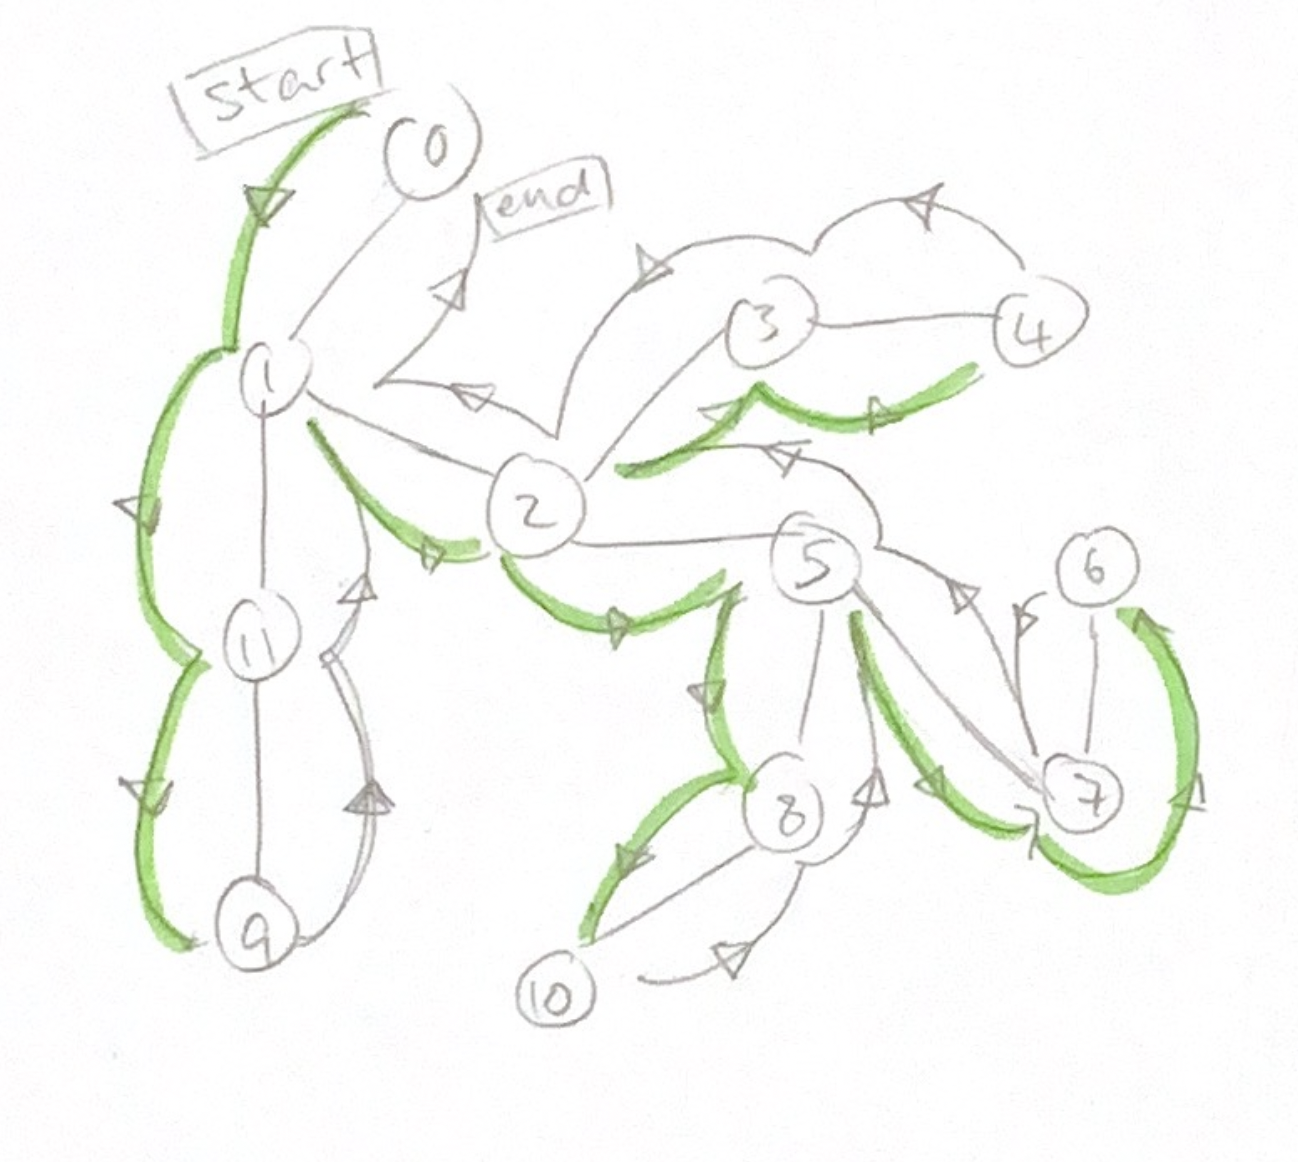
\includegraphics[scale=0.40]{q1pic.png}
\end{minipage}

\newpage
\section{Question 2.}
There are two types of professional wrestlers: “good guys” and “bad guys”. Between any pair of professional wrestlers, there may or may not be a rivalry. Suppose we have n professional wrestlers, and we have a list of r pairs of wrestlers for which there are rivalries. Give an O(n + r)-time algorithm that determines whether it is possible to designate some of the wrestlers as “good guys” and the remainder as “bad guys” such that each rivalry is between a good guy and a bad guy. If it is possible to perform such a designation, your algorithm should produce it.
\\\\
Wrestlers are vertices and rivalries are edges. Designating a wrestler one of two labels (good or bad guy) such that each edge (rivalry) is between nodes of different labels is equivalent to testing for bipartiteness. As shown in lecture, this is equivalent to finding an odd cycle, and can be done with a tree traversal where vertices are marked with opposite labels as their "parent" vertex in the traversal tree. If we mark a vertex and find a neighbor with that same label, then the graph is not bipartite.
\begin{algorithm}
\begin{algorithmic}[1]

\Procedure{LabelWrestlerAndTheirRivals}{start: vertex to begin with, label: starting label}
	\State start.label $\gets$ label
	\For{neighbor in neighbors(start)}
		\If{label == neighbor.label} \Comment{odd cycle detected, abort}
			\State \Return \text{false}
		\EndIf	
		\State successful $\gets$ \Call{LabelWrestlerAndTheirRivals}{neighbor, opposite(label)}
		\If{not successful}
			\State \Return \text{false}
		\EndIf
	\EndFor
	\State \Return \text{true}
\EndProcedure
\State
\Procedure{LabelGoodOrBad}{wrestlers: array of nodes}
	\For{wrestler in wrestlers} \Comment{initialize all labels as None}
		\State wrestler.label $\gets$ None
	\EndFor
	
	\For{wrestler in wrestlers}
		\If{wrestler.label is None}
			\State successful $\gets$ \Call{LabelWrestlerAndTheirRivals}{wrestler, good}
			\If{not successful}
				\State \Return \text{false}
			\EndIf
		\EndIf
	\EndFor
	\State \Return \text{true}
\EndProcedure


\end{algorithmic}
\end{algorithm}

\newpage
\section{Question 3.}
Explain how both Prim’s and Kruskal’s Minimum Spanning Tree algorithm works on the graph below and print out the edges and its weight as you add it to your MST set. Assume that your source vertex is 0 and that your adjacency list is ordered in decreasing numerical values.

\end{document}
